\documentclass{standalone}
\usepackage{tikz}
\usetikzlibrary{patterns, positioning}
\usepackage[sfdefault]{ClearSans} %% option 'sfdefault' activates Clear Sans as the default text font
\usepackage[T1]{fontenc}

\begin{document}
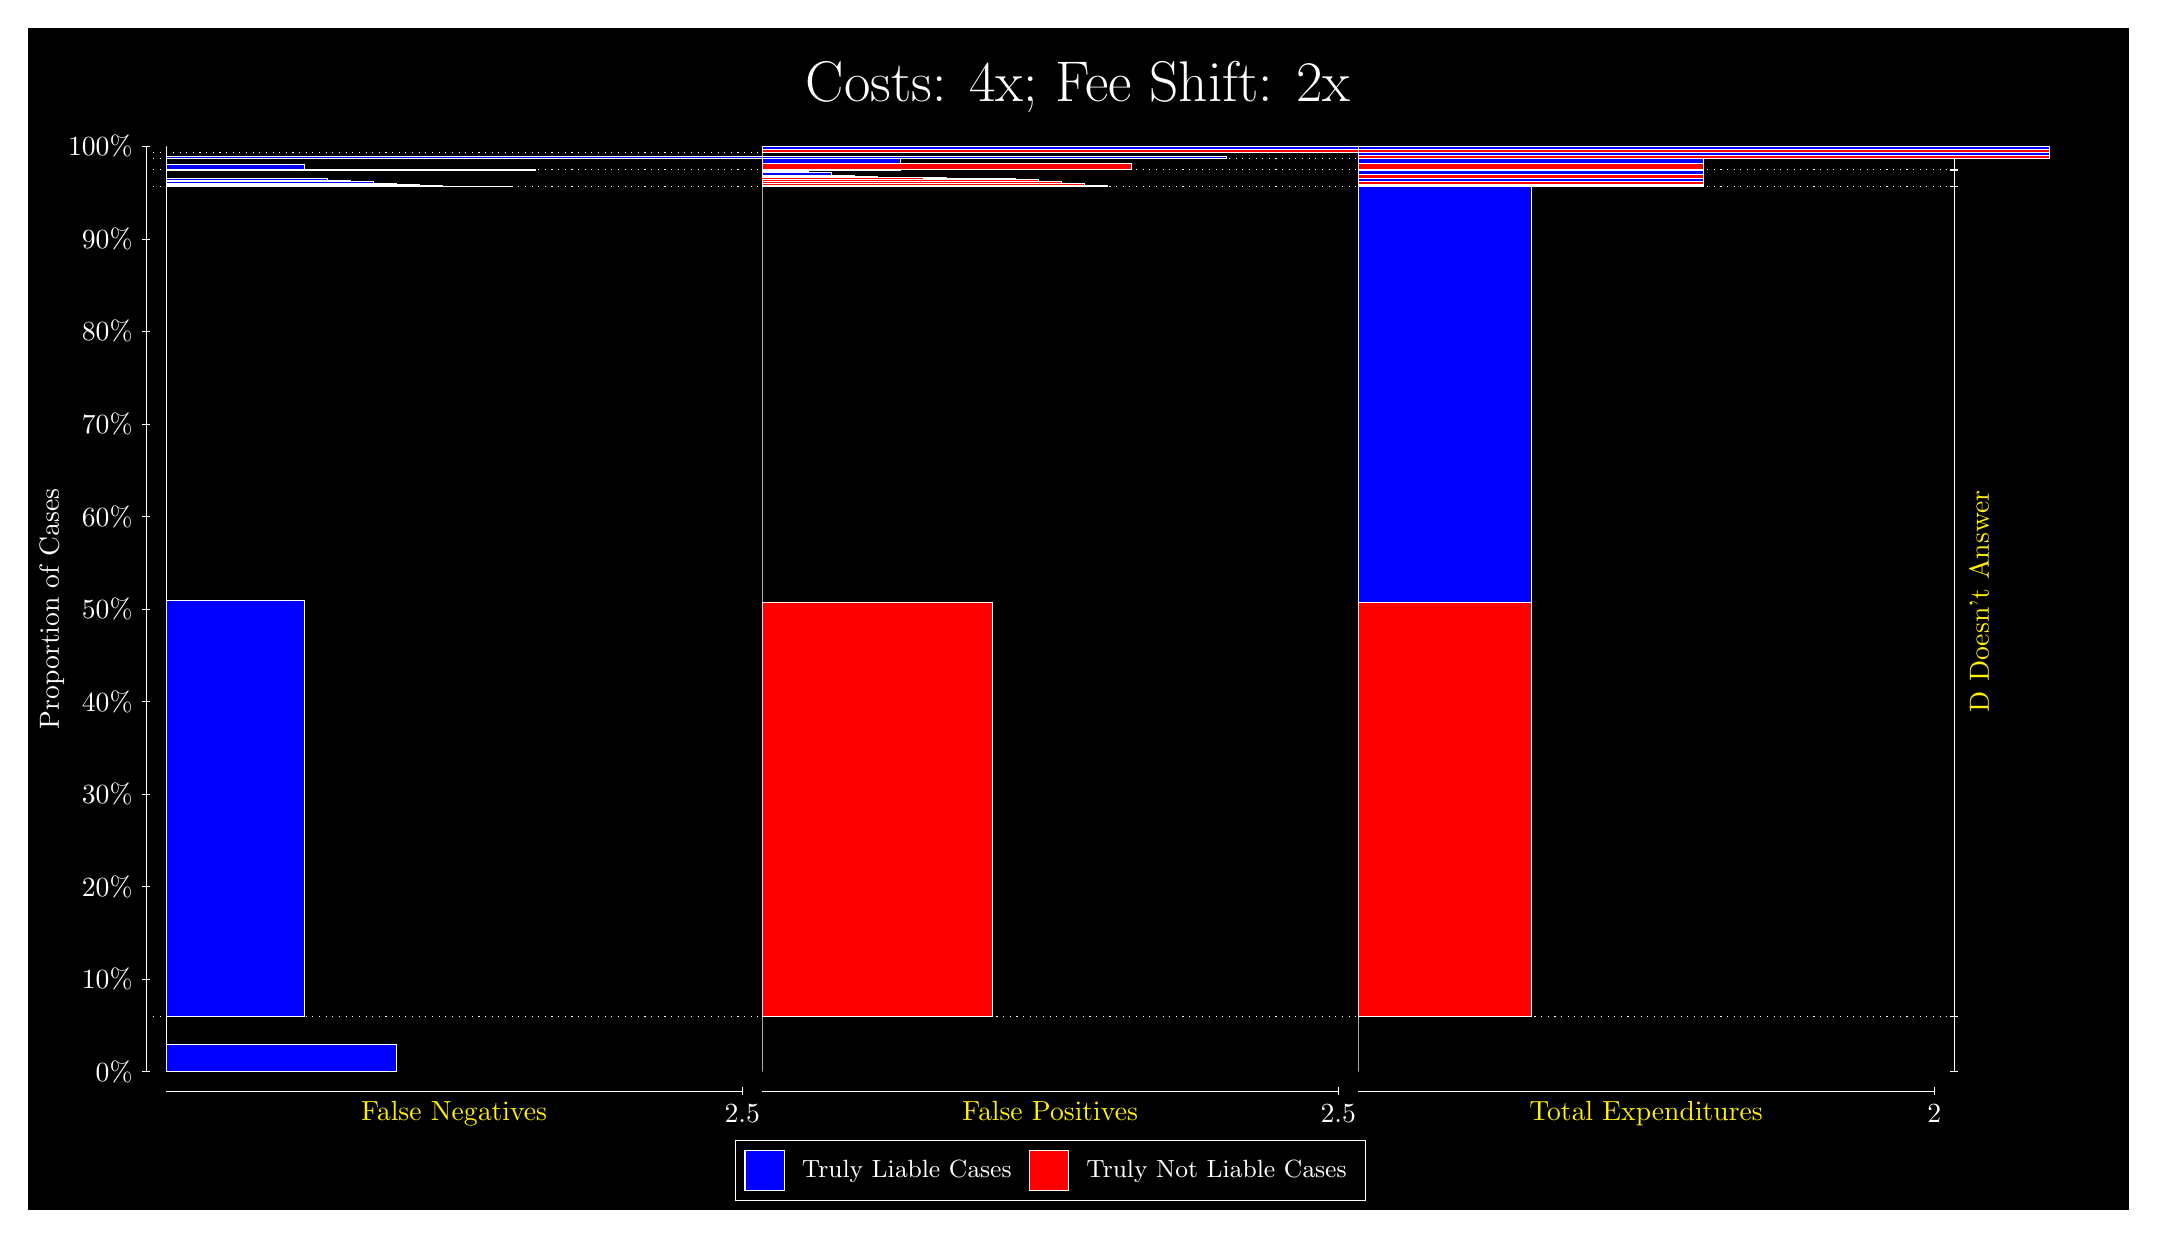
\begin{tikzpicture}
\draw[fill=black] (0,0) rectangle (26.667,15);
\draw[text=white] (0,13.5) rectangle (26.667,15) node[midway] {\huge Costs: 4x; Fee Shift: 2x};
\draw[white, very thin] (1.5,1.75) -- (1.5,13.5);
\node[rotate=90, text=white, anchor=center] at (0.3, 7.625) {Proportion of Cases};
\draw[white, very thin] (1.45,1.75) -- (1.55,1.75);
\node[text=white, anchor=east] at (1.45, 1.75) {0\%};
\draw[white, very thin] (1.45,2.925) -- (1.55,2.925);
\node[text=white, anchor=east] at (1.45, 2.925) {10\%};
\draw[white, very thin] (1.45,4.1) -- (1.55,4.1);
\node[text=white, anchor=east] at (1.45, 4.1) {20\%};
\draw[white, very thin] (1.45,5.275) -- (1.55,5.275);
\node[text=white, anchor=east] at (1.45, 5.275) {30\%};
\draw[white, very thin] (1.45,6.45) -- (1.55,6.45);
\node[text=white, anchor=east] at (1.45, 6.45) {40\%};
\draw[white, very thin] (1.45,7.625) -- (1.55,7.625);
\node[text=white, anchor=east] at (1.45, 7.625) {50\%};
\draw[white, very thin] (1.45,8.8) -- (1.55,8.8);
\node[text=white, anchor=east] at (1.45, 8.8) {60\%};
\draw[white, very thin] (1.45,9.975) -- (1.55,9.975);
\node[text=white, anchor=east] at (1.45, 9.975) {70\%};
\draw[white, very thin] (1.45,11.15) -- (1.55,11.15);
\node[text=white, anchor=east] at (1.45, 11.15) {80\%};
\draw[white, very thin] (1.45,12.325) -- (1.55,12.325);
\node[text=white, anchor=east] at (1.45, 12.325) {90\%};
\draw[white, very thin] (1.45,13.5) -- (1.55,13.5);
\node[text=white, anchor=east] at (1.45, 13.5) {100\%};

\draw[white, very thin] (24.457,1.75) -- (24.457,13.5);
\draw[white, very thin] (24.407,1.75) -- (24.507,1.75);
\node[anchor=west] at (24.407, 1.75) {};
\draw[white, very thin] (24.407,2.4514) -- (24.507,2.4514);
\node[anchor=west] at (24.407, 2.4514) {};
\draw[white, very thin] (24.407,12.99) -- (24.507,12.99);
\node[anchor=west] at (24.407, 12.99) {};
\draw[white, very thin] (24.407,13.201) -- (24.507,13.201);
\node[anchor=west] at (24.407, 13.201) {};
\draw[white, very thin] (24.407,13.211) -- (24.507,13.211);
\node[anchor=west] at (24.407, 13.211) {};
\draw[white, very thin] (24.407,13.346) -- (24.507,13.346);
\node[anchor=west] at (24.407, 13.346) {};
\draw[white, very thin] (24.407,13.424) -- (24.507,13.424);
\node[anchor=west] at (24.407, 13.424) {};
\draw[white, very thin] (24.407,13.5) -- (24.507,13.5);
\node[anchor=west] at (24.407, 13.5) {};

\draw[white, very thin, fill=blue] (1.75,1.75) rectangle (4.6775,2.1007);
\draw[white, very thin, fill=red] (1.75,2.1007) rectangle (1.75,2.4514);
\draw[white, very thin, fill=blue] (1.75,2.4514) rectangle (3.5065,7.7379);
\draw[white, very thin, fill=red] (1.75,7.7379) rectangle (1.75,12.99);
\draw[white, very thin, fill=blue] (1.75,12.99) rectangle (6.1413,12.992);
\draw[white, very thin, fill=blue] (1.75,12.992) rectangle (5.8486,12.993);
\draw[white, very thin, fill=blue] (1.75,12.993) rectangle (5.5558,12.996);
\draw[white, very thin, fill=blue] (1.75,12.996) rectangle (5.2631,12.999);
\draw[white, very thin, fill=blue] (1.75,12.999) rectangle (4.9703,13.013);
\draw[white, very thin, fill=blue] (1.75,13.013) rectangle (4.6775,13.025);
\draw[white, very thin, fill=blue] (1.75,13.025) rectangle (4.3848,13.055);
\draw[white, very thin, fill=blue] (1.75,13.055) rectangle (4.092,13.075);
\draw[white, very thin, fill=blue] (1.75,13.075) rectangle (3.7993,13.088);
\draw[white, very thin, fill=red] (1.75,13.088) rectangle (1.75,13.201);
\draw[white, very thin, fill=blue] (1.75,13.201) rectangle (6.4341,13.206);
\draw[white, very thin, fill=red] (1.75,13.206) rectangle (1.75,13.211);
\draw[white, very thin, fill=blue] (1.75,13.211) rectangle (3.5065,13.274);
\draw[white, very thin, fill=red] (1.75,13.274) rectangle (1.75,13.346);
\draw[white, very thin, fill=blue] (1.75,13.346) rectangle (15.217,13.379);
\draw[white, very thin, fill=red] (1.75,13.379) rectangle (1.75,13.424);
\draw[white, very thin, fill=red] (1.75,13.424) rectangle (1.75,13.461);
\draw[white, very thin, fill=blue] (1.75,13.461) rectangle (1.75,13.5);
\draw[white, very thin, fill=red] (9.3189,1.75) rectangle (9.3189,2.1007);
\draw[white, very thin, fill=blue] (9.3189,2.1007) rectangle (9.3189,2.4514);
\draw[white, very thin, fill=red] (9.3189,2.4514) rectangle (12.246,7.7037);
\draw[white, very thin, fill=blue] (9.3189,7.7037) rectangle (9.3189,12.99);
\draw[white, very thin, fill=red] (9.3189,12.99) rectangle (13.71,13.003);
\draw[white, very thin, fill=red] (9.3189,13.003) rectangle (13.417,13.026);
\draw[white, very thin, fill=red] (9.3189,13.026) rectangle (13.125,13.062);
\draw[white, very thin, fill=red] (9.3189,13.062) rectangle (12.832,13.077);
\draw[white, very thin, fill=red] (9.3189,13.077) rectangle (12.539,13.093);
\draw[white, very thin, fill=red] (9.3189,13.093) rectangle (12.246,13.097);
\draw[white, very thin, fill=red] (9.3189,13.097) rectangle (11.954,13.1);
\draw[white, very thin, fill=red] (9.3189,13.1) rectangle (11.661,13.102);
\draw[white, very thin, fill=red] (9.3189,13.102) rectangle (11.368,13.104);
\draw[white, very thin, fill=blue] (9.3189,13.104) rectangle (10.783,13.116);
\draw[white, very thin, fill=blue] (9.3189,13.116) rectangle (10.49,13.136);
\draw[white, very thin, fill=blue] (9.3189,13.136) rectangle (10.197,13.167);
\draw[white, very thin, fill=blue] (9.3189,13.167) rectangle (9.9044,13.179);
\draw[white, very thin, fill=blue] (9.3189,13.179) rectangle (9.6116,13.193);
\draw[white, very thin, fill=blue] (9.3189,13.193) rectangle (9.3189,13.201);
\draw[white, very thin, fill=red] (9.3189,13.201) rectangle (11.075,13.207);
\draw[white, very thin, fill=blue] (9.3189,13.207) rectangle (9.3189,13.211);
\draw[white, very thin, fill=red] (9.3189,13.211) rectangle (14.003,13.282);
\draw[white, very thin, fill=blue] (9.3189,13.282) rectangle (11.075,13.346);
\draw[white, very thin, fill=red] (9.3189,13.346) rectangle (9.3189,13.39);
\draw[white, very thin, fill=blue] (9.3189,13.39) rectangle (9.3189,13.424);
\draw[white, very thin, fill=red] (9.3189,13.424) rectangle (22.786,13.461);
\draw[white, very thin, fill=blue] (9.3189,13.461) rectangle (19.858,13.5);
\draw[white, very thin, fill=red] (16.888,1.75) rectangle (16.888,2.1007);
\draw[white, very thin, fill=blue] (16.888,2.1007) rectangle (16.888,2.4514);
\draw[white, very thin, fill=red] (16.888,2.4514) rectangle (19.083,7.7037);
\draw[white, very thin, fill=blue] (16.888,7.7037) rectangle (19.083,12.99);
\draw[white, very thin, fill=red] (16.888,12.99) rectangle (21.279,13.007);
\draw[white, very thin, fill=blue] (16.888,13.007) rectangle (21.279,13.02);
\draw[white, very thin, fill=red] (16.888,13.02) rectangle (21.279,13.059);
\draw[white, very thin, fill=blue] (16.888,13.059) rectangle (21.279,13.092);
\draw[white, very thin, fill=red] (16.888,13.092) rectangle (21.279,13.151);
\draw[white, very thin, fill=blue] (16.888,13.151) rectangle (21.279,13.201);
\draw[white, very thin, fill=red] (16.888,13.201) rectangle (21.279,13.207);
\draw[white, very thin, fill=blue] (16.888,13.207) rectangle (21.279,13.211);
\draw[white, very thin, fill=red] (16.888,13.211) rectangle (21.279,13.282);
\draw[white, very thin, fill=blue] (16.888,13.282) rectangle (21.279,13.346);
\draw[white, very thin, fill=red] (16.888,13.346) rectangle (25.67,13.39);
\draw[white, very thin, fill=blue] (16.888,13.39) rectangle (25.67,13.424);
\draw[white, very thin, fill=red] (16.888,13.424) rectangle (25.67,13.461);
\draw[white, very thin, fill=blue] (16.888,13.461) rectangle (25.67,13.5);
\draw[white, dotted] (1.5,2.4514) -- (24.457,2.4514);
\draw[white, dotted] (1.5,12.99) -- (24.457,12.99);
\draw[white, dotted] (1.5,13.201) -- (24.457,13.201);
\draw[white, dotted] (1.5,13.211) -- (24.457,13.211);
\draw[white, dotted] (1.5,13.346) -- (24.457,13.346);
\draw[white, dotted] (1.5,13.424) -- (24.457,13.424);
\draw[white, very thin] (1.75,1.5) -- (9.0689,1.5);
\node[text=yellow, anchor=north] at (5.4094, 1.5) {False Negatives};
\draw[white, very thin] (9.0689,1.45) -- (9.0689,1.55);
\node[text=white, anchor=north] at (9.0689, 1.45) {2.5};

\draw[white, very thin] (9.3189,1.5) -- (16.638,1.5);
\node[text=yellow, anchor=north] at (12.978, 1.5) {False Positives};
\draw[white, very thin] (16.638,1.45) -- (16.638,1.55);
\node[text=white, anchor=north] at (16.638, 1.45) {2.5};

\draw[white, very thin] (16.888,1.5) -- (24.207,1.5);
\node[text=yellow, anchor=north] at (20.547, 1.5) {Total Expenditures};
\draw[white, very thin] (24.207,1.45) -- (24.207,1.55);
\node[text=white, anchor=north] at (24.207, 1.45) {2};


\node[text=yellow, centered, rotate=90] at (24.777, 7.7208) {D Doesn't Answer};






\draw (12.978300999999998,1.5) node[draw=none] (baseCoordinate) {};
\begin{scope}[align=center]
        \matrix[scale=0.5, draw=white, below=0.5cm of baseCoordinate, nodes={draw}, column sep=0.1cm]{
            \node[rectangle, draw, minimum width=0.5cm, minimum height=0.5cm, fill=blue] {}; &
            \node[draw=none, font=\small, text=white] (B) {Truly Liable Cases}; &
            \node[rectangle, draw, minimum width=0.5cm, minimum height=0.5cm, fill=red] {}; &
            \node[draw=none, font=\small, text=white] (B) {Truly Not Liable Cases}; \\
            };
\end{scope}

\end{tikzpicture}
\end{document}